\section*{Experiment 3}
%signal was 3.2 kHz
Differential amplifiers are often used in AC contexts, where the output voltage often has to change rapidly depending on the inputs. One case is when a unity-gain amplifier must pass a square wave. We saw in pre-lab 9 that an improved diff amp with a small capacitive load can only change \Vout so quickly, and in this experiment we tested the step response of the diff amp to both large and small steps, with a $1 nF$ capacitor parallel to the feedback loop. We saw that given a small step, \Vout takes a first-order approach to \Vin, and extracted time constants for both the up- and down-swings. We also saw that given a large step, \Vout approaches \Vin linearly, and we extracted values for the slew rate for both the up- and down-swings.

\subsection*{Small Signal Analysis}

We first started by sending a $3.2 kHz$ square wave into the unity-gain follower, with a peak to peak voltage of 30 mV. This low amplitude ensured that we would see that small signal response of the unity-gain buffer. We used the oscilloscope to take data for \Vin and \Vout, and then extracted experimental values for time constants. We also used the value of \Gm we extracted in experiment 2, along with the known value of the capacitor, to derive a theoretical value for the time constant $\tau$.

Recalling pre-lab 9, we know that \Vout follows \Vin according to the following equation:

\begin{equation}
V_{out} = V_{in} - V_{out}(0)e^{-\frac{G_m}{C}t}
\end{equation}

Where \Gm is the incremental transconductance gain of the circuit and $C$ is the capacitance of the capactive load to the circuit. We define our time constant $\tau$ as:

\begin{equation}
\tau = \frac{C}{G_m}
\end{equation}	

Given our extracted value for \Gm from experiment 2 and the $1 nF$ capacitor, we expect our theoretical time constant to have a value of $4.22 \times 10^{-6}$ seconds. In figure \ref{fig:exp3p2}, we plotted the experimental results from our small-signal experiment along with theoretical fits using our theoretical time constant. We also extracted time constants for the up- and down-swing using the 63\% trick, and plotted curves for using those values of $\tau$ as well.

\begin{figure}[H]
\centering
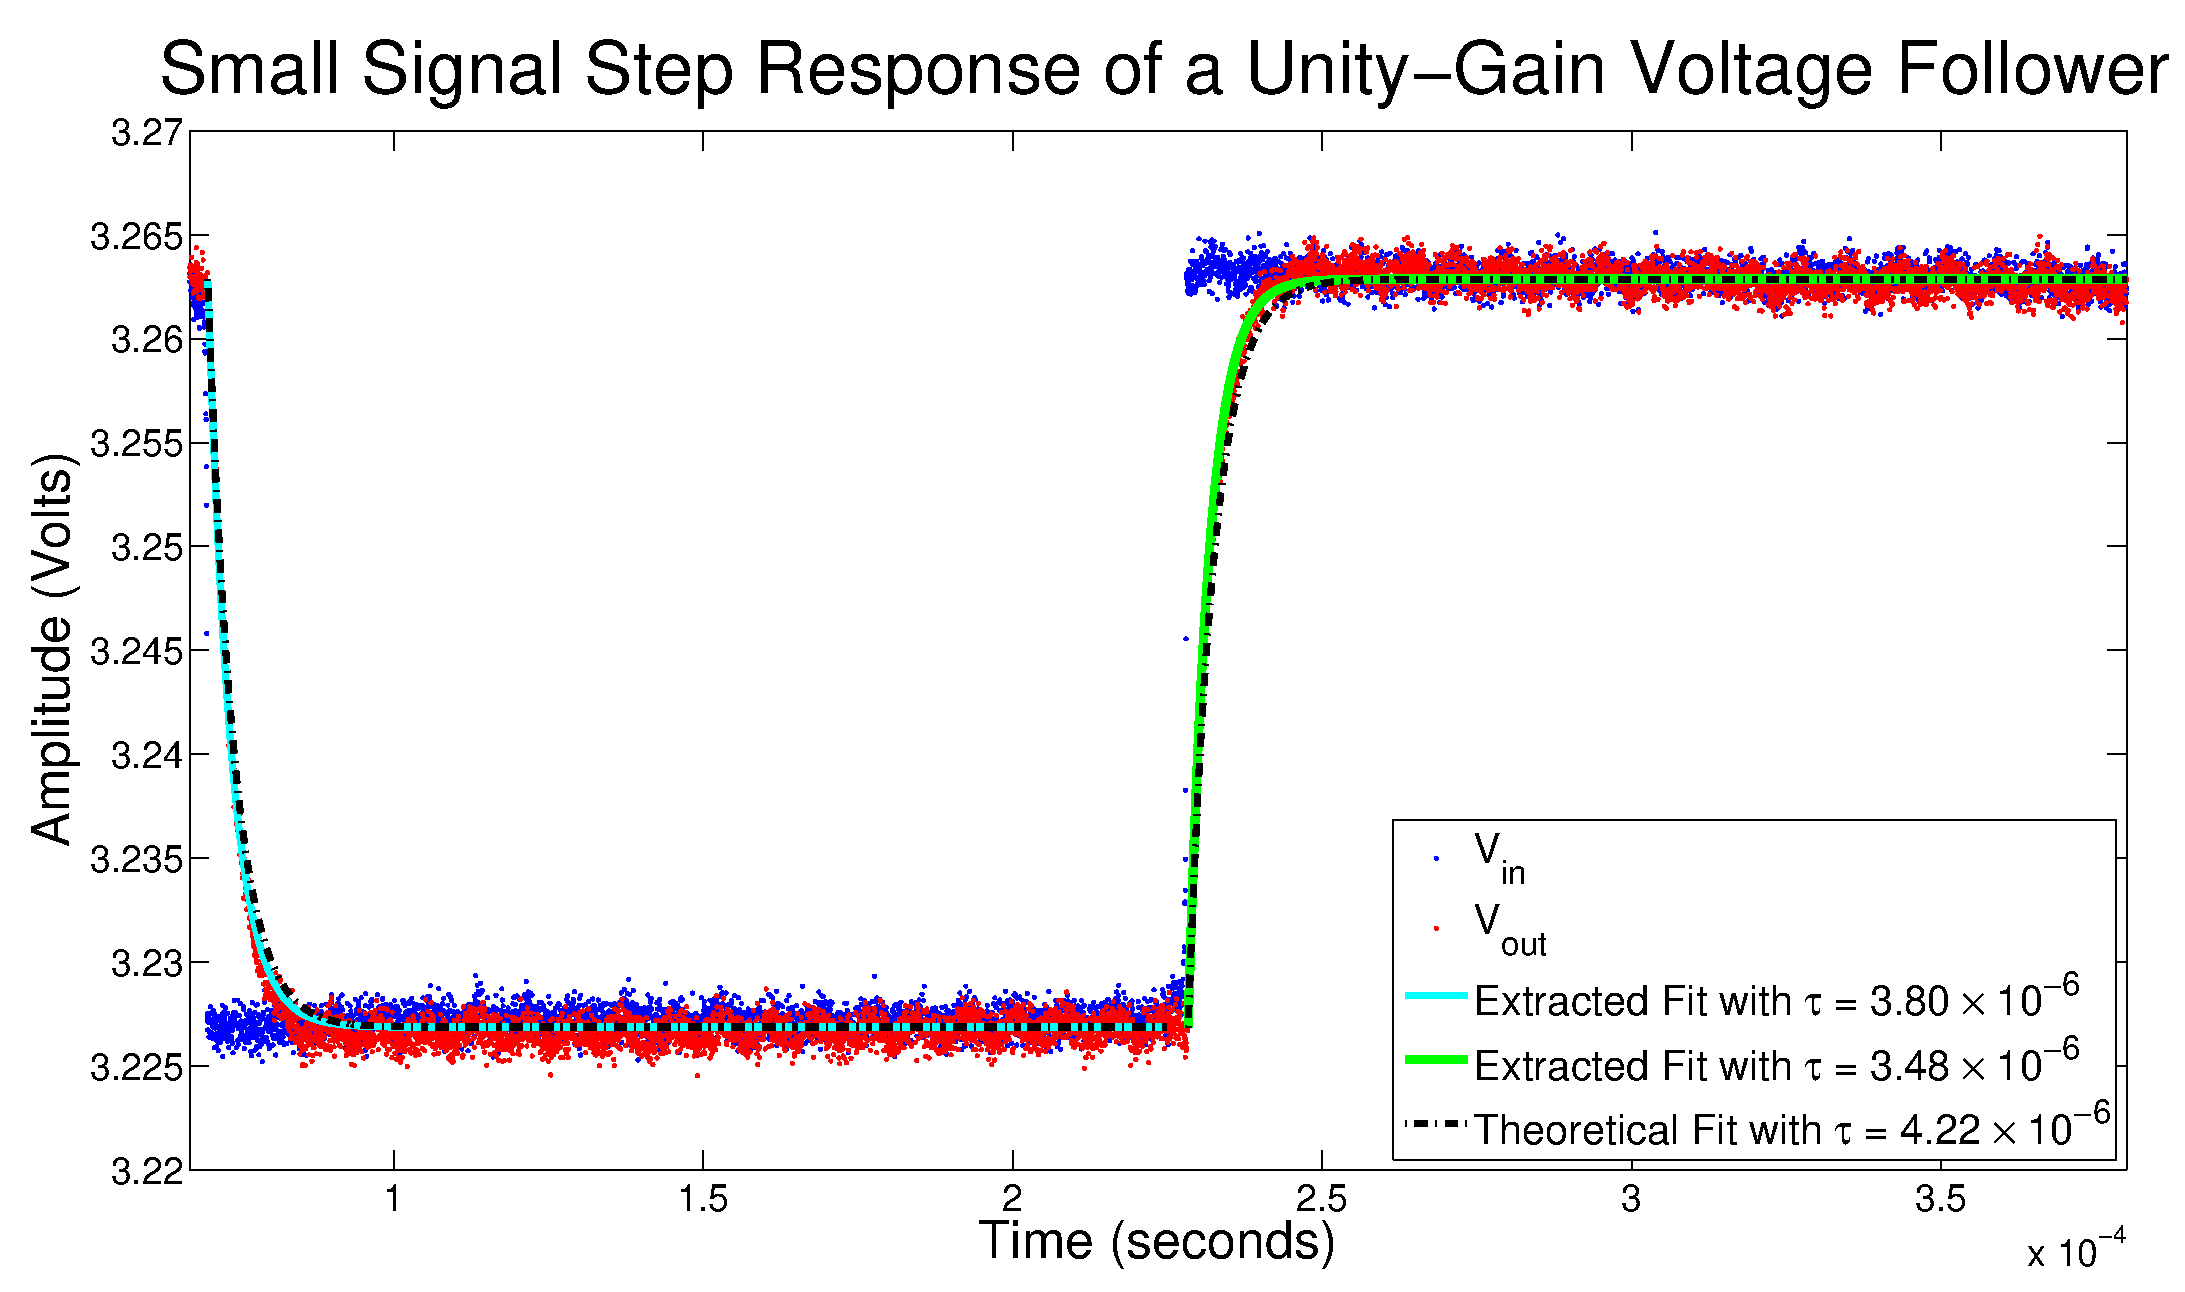
\includegraphics[width=\linewidth]{../Figures/Exp3P2.eps}
\caption{Small-signal step response of a unity-gain voltage follower. We can see that \Vout follows a first-order approach to \Vin. The following is slightly asymmetrical, with extracted time constants that are about 10\% apart.}
\label{fig:exp3p2}
\end{figure}

We first saw that the down- and up-swing of \Vout following a first-order approach to \Vin, which is the kind of approach we expect for small steps. For the down-swinging change in \Vout, we found that $\tau = 3.8 \times 10^{-6}$, and for the up-swing change in \Vout we found that $\tau = 3.48 \times 10^{-6}$. The experimentally-derived values for $\tau$ deviate from our theoretical value by an average of 15\%, which is pretty close considering the magnitude of the time constant. We expect that the slight difference (about 10\%) between the down-swing and up-swing time constants could be due to the different inherenet properties of the pMOS and nMOS transistors used in the current mirrors that generate \Vout. Small differences in these transistors could cause \Vout to deviate slightly when $V_{dm} = 0$, which would in turn change how \Vout approaches \Vin when increasing or decreasing.

\subsection*{Large Signal Analysis}

% Is the response symmetrical? You will probably notice that the output
% of the amplifier follows a linear trajectory in time over most of its response to the large input
% step. This behavior is called slewing, and the constant rate of change of the output voltage
% with respect to time is called the slew rate of the amplifier. Extract a slew rate for both for
% the up-going and for the down-going output transitions. How do these compare with those
% which you compute from the load capacitance and the limiting values of the output current?
% In your report, include a single plot showing both scope traces along with the extracted slew
% rates.

\begin{figure}[H]
\centering
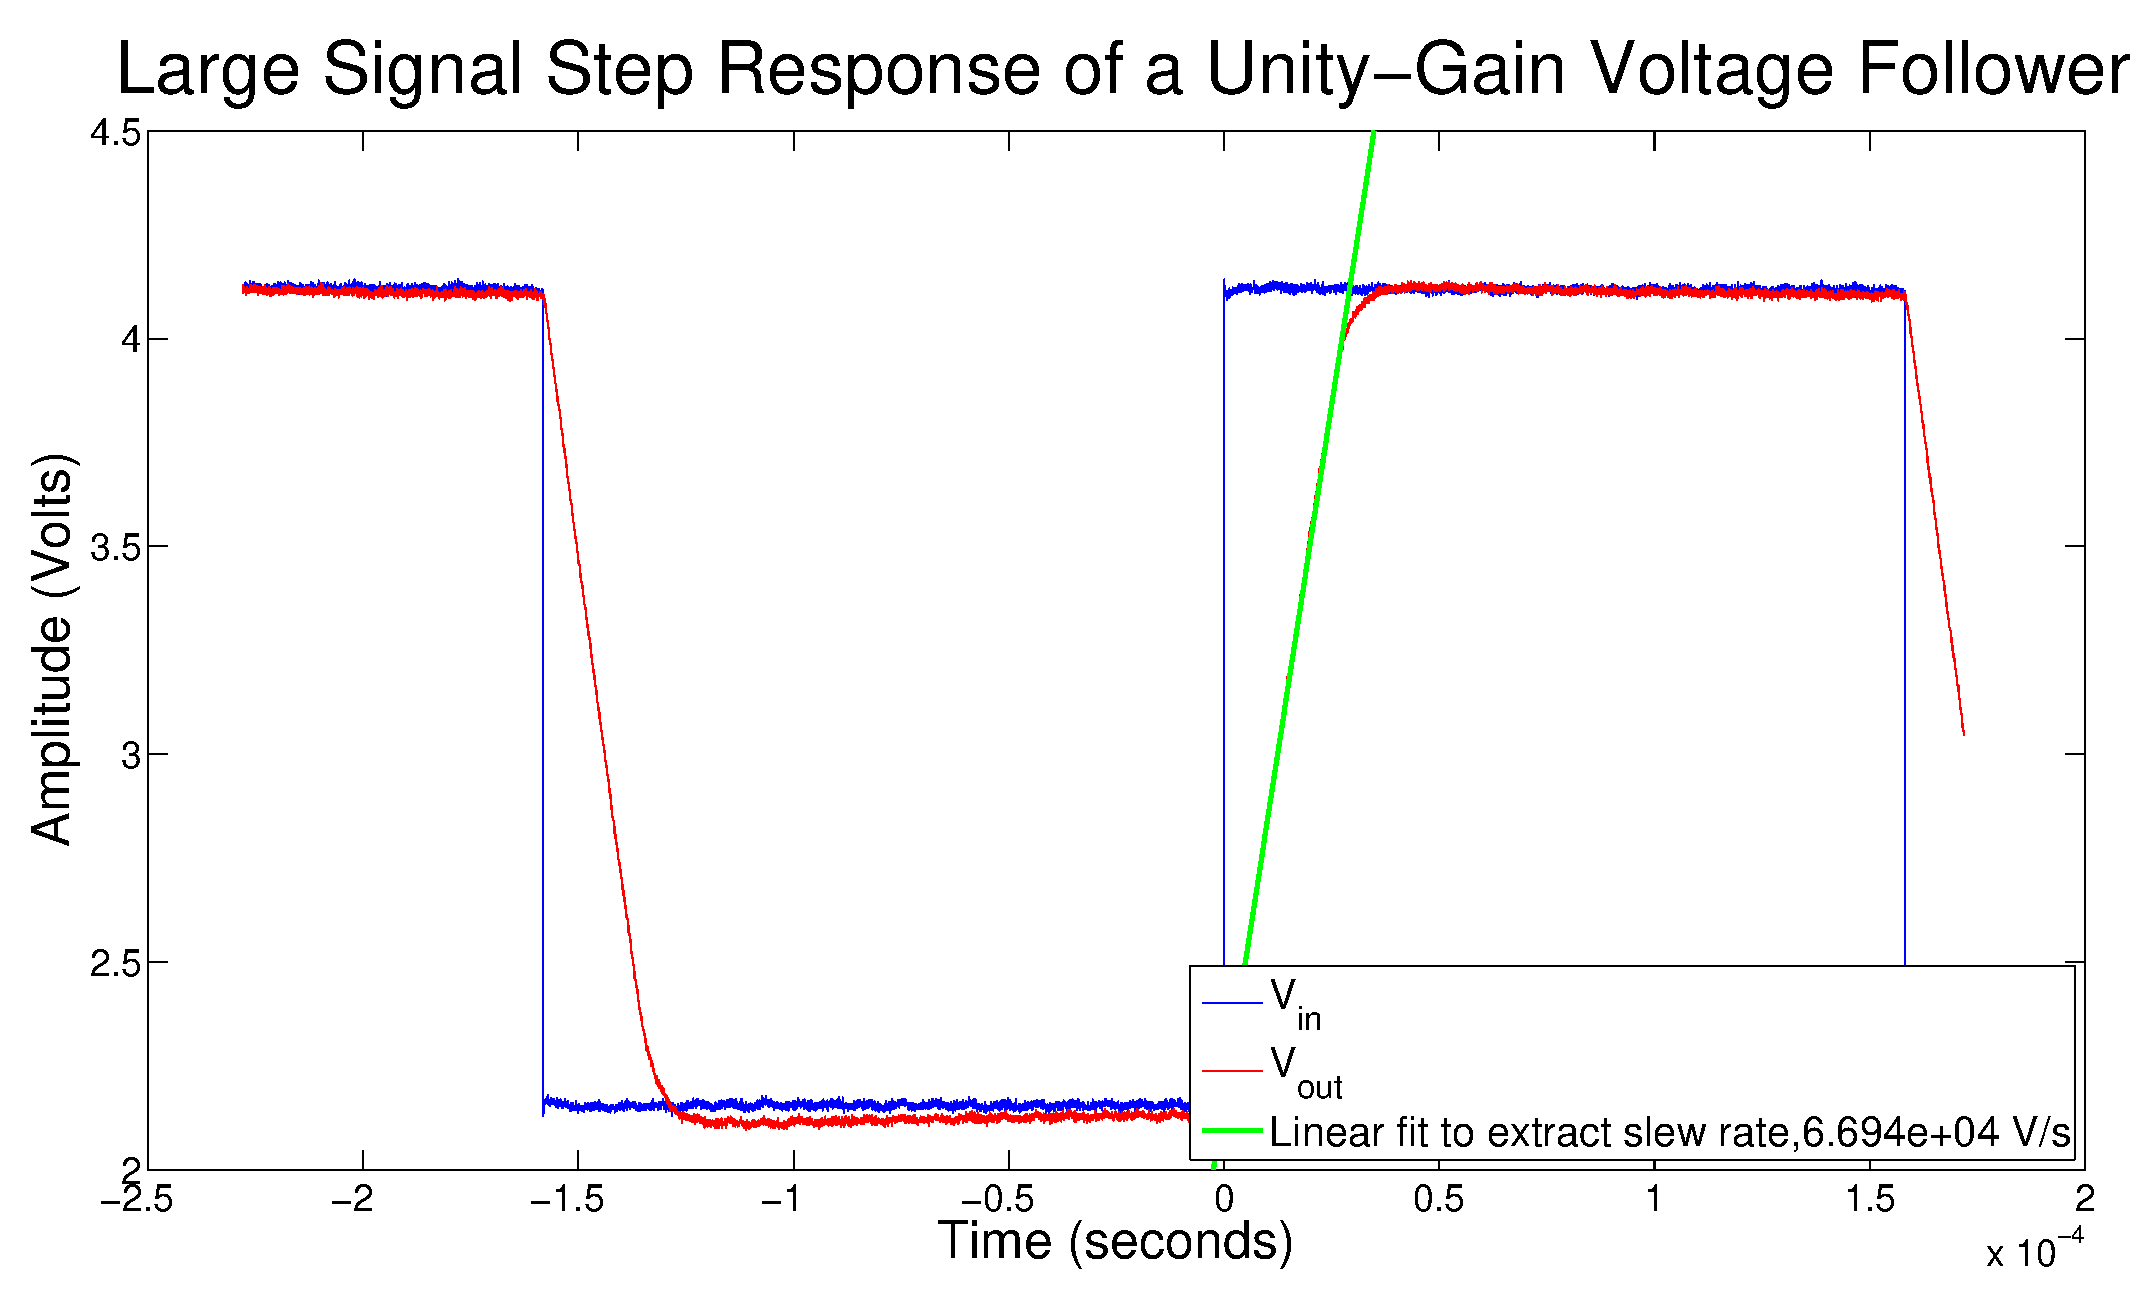
\includegraphics[width=\linewidth]{../Figures/Exp3P1.eps}
\caption{}
\label{fig:exp3p1}
\end{figure}